\documentclass[10pt]{article}
\usepackage{tmlr}

% --- Core Math & Typography Packages ---
\usepackage{amsmath,amssymb,amsfonts,amsthm}
\usepackage{mathtools}
\usepackage{microtype}        % professional paragraph microtypography
\usepackage{booktabs}
\usepackage{multirow}
\usepackage{array}
\usepackage{graphicx}
\usepackage{xcolor}
\usepackage{enumitem}
\usepackage{pifont}
\usepackage{url}
\usepackage[colorlinks=true,linkcolor=blue!80!black,citecolor=blue!80!black,urlcolor=blue!80!black]{hyperref}
\usepackage{natbib}

% --- Table & Paragraph Settings ---
\renewcommand{\arraystretch}{1.12}

% Standard TMLR float spacing

% --- Theorem & Definition Helpers ---
\theoremstyle{definition}
\newtheorem{definition}{Definition}
\newtheorem{proposition}{Proposition}

\newcommand{\cmark}{\textcolor{green!60!black}{\ding{51}}}
\newcommand{\xmark}{\textcolor{red!70!black}{\ding{55}}}

% --- Vertical Spacing: 3x Whitespace on Page 1, Balanced Page Margins & Vertically Centered Footer ---
\setlength{\topmargin}{-0.30in}
\setlength{\headsep}{14pt}
\setlength{\textheight}{9.15in}
\setlength{\footskip}{30pt}
\setlength{\aftertitskip}{54pt}

% --- Formula Spacing: Distinct Space Above & Below Display Equations ---
\setlength{\abovedisplayskip}{12pt plus 3pt minus 2pt}
\setlength{\belowdisplayskip}{12pt plus 3pt minus 2pt}
\setlength{\abovedisplayshortskip}{8pt plus 3pt minus 2pt}
\setlength{\belowdisplayshortskip}{8pt plus 3pt minus 2pt}

% --- Table & Float Spacing: Distinct Space Above & Below Tables & Captions ---
\setlength{\floatsep}{18pt plus 3pt minus 2pt}
\setlength{\textfloatsep}{18pt plus 3pt minus 2pt}
\setlength{\intextsep}{18pt plus 3pt minus 2pt}
\setlength{\abovecaptionskip}{10pt plus 2pt minus 2pt}
\setlength{\belowcaptionskip}{8pt plus 2pt minus 1pt}

\makeatletter
\def\@maketitle{\vbox{\hsize\textwidth
\vskip 30pt
{\LARGE\bfseries \@title\par}\vskip \aftertitskip
\if@accepted
    \if@preprint
        \@startauthor \@author \@endauthor
    \else
        \@startauthor \@author \\ \\ {\bf Reviewed on OpenReview:} \openreview \@endauthor
    \fi
\else
    \@startauthor Anonymous authors\\Paper under double-blind review \@endauthor
\fi
\vskip 54pt}}
\makeatother

% --- Title Block ---
\title{CRBench: A Method-Agnostic, Resource-Aware \\ Evaluation Framework for Long-Context \\ Large Language Models\thanks{Large language models were used as assistive writing tools for stylistic editing and drafting under the authors' direct supervision; the authors take full responsibility for all content, experimental methodology, and scientific claims.}}

\author{\name Anonymous authors \\
        \addr Paper under double-blind review --- Technical Report}

\begin{document}

\maketitle

% ==============================================================================
% ABSTRACT
% ==============================================================================
\begin{abstract}
As Large Language Models (LLMs) expand context windows beyond 32K, 128K, and 1M tokens, the Key-Value (KV) cache becomes a primary operational bottleneck during autoregressive inference. While diverse compression paradigms have emerged---including quantization, token eviction, pooling, low-rank projection, and factorized representations---current evaluation practices often separate task accuracy from physical resource usage and report results across heterogeneous tasks, models, and accounting conventions.

We introduce CRBench, a method-agnostic, resource-aware evaluation framework for rigorously benchmarking long-context LLMs and context-compression techniques. CRBench formulates evaluation around an atomic query-level primitive that pairs every compressed execution with an uncompressed dense baseline on the identical prompt. The framework decouples evaluation into two complementary tracks: Part~1 measures algorithmic representation utility ($\mathcal{S}_{\text{res}}$) by combining absolute task quality with effective memory savings, where effective bits-per-element ($b_{\text{eff}}$) accounts for representation metadata and storage overheads; Part~2 measures hardware system serving utility ($\mathcal{S}_{\text{sys}}$) using physical time-to-first-token (TTFT), decode throughput, peak VRAM, and a baseline-relative hardware efficiency multiplier.

We evaluate seven context-compression methods alongside an uncompressed dense reference across three foundation models (Gemma~4 E2B, Gemma~4 E4B, and Qwen2.5~7B), spanning 3,150 queries across five long-context tasks from 2K to 128K tokens on NVIDIA RTX hardware. Empirical results show that: (1)~KIVI-style INT4 quantization achieves the highest cross-model system score (mean $\mathcal{S}_{\text{sys}} = 70.3$) with near-baseline hardware efficiency ($\phi \ge 0.96\times$); (2)~SnapKV provides strong algorithmic utility ($\mathcal{S}_{\text{res}} = 60.8$ on Gemma~4 E4B) but incurs substantial prefill overhead under un-fused attention pooling (TTFT = 83.4\,s at 32K); (3)~DKV-Mid operates at 5.00--5.84 effective bits-per-element across the three models, with 44.7--55.3\% mean task accuracy; and (4)~all evaluated methods, including dense FP16, perform near zero on multi-step variable tracking, suggesting that this task is substantially limited by the underlying base models rather than KV compression. CRBench is released with an extensible adapter API and reproducible evaluation pipeline.
\end{abstract}

% ==============================================================================
% 1. INTRODUCTION
% ==============================================================================
\section{Introduction}
\label{sec:introduction}

Modern Large Language Models (LLMs) have achieved remarkable breakthroughs across multi-document synthesis, complex multi-hop question answering, repository-scale code generation, and autonomous agent workflows~\citep{brown2020language,achiam2023gpt4,touvron2023llama,bai2023qwen}. These capabilities rely on long-context processing, expanding context horizons from 2,048 tokens to 32,768, 131,072, and beyond~\citep{reid2024gemini,deepseek2024v2}.

However, contextual expansion is fundamentally bounded by the memory footprint of the Key-Value (KV) cache in standard Transformer self-attention architectures~\citep{vaswani2017attention}. Because standard attention caches intermediate key and value tensor representations for every historical token across all layers and attention heads, KV cache memory scales linearly with sequence length $L$ and batch size $B$:
\begin{equation}
\label{eq:kv_size_intro}
M_{\text{KV}} = 2 \times N_{\text{layers}} \times N_{\text{kv\_heads}} \times d_{\text{head}} \times L \times B \times \text{sizeof}(\text{dtype}) \quad [\text{bytes}]
\end{equation}
For a representative 8-billion parameter model (e.g., Llama-3.1-8B with 32 layers, 8 Key-Value heads under Grouped-Query Attention, and head dimension 128 in 16-bit precision), a single batch-1 128K-token sequence ($L = 131{,}072$) requires exactly $16.0\,\text{GiB}$ ($17.18\,\text{GB}$) of memory purely for the KV cache ($2 \times 32 \times 8 \times 128 \times 131{,}072 \times 2\,\text{bytes}$)---exceeding the model's static weight footprint and exhausting consumer GPU VRAM.

To address this severe memory wall, the machine learning community has introduced a diverse taxonomy of context compression paradigms:
\begin{enumerate}[leftmargin=*,itemsep=1.5pt]
    \item \textbf{KV Cache Quantization}: Low-precision numerical formats (FP8, INT8, INT4, INT2) with per-channel or group-wise dynamic scaling~\citep{dettmers2022llmint8,hooper2024kvquant,liu2024kivi}.
    \item \textbf{KV Cache Eviction \& Sparsification}: Attention sinks and dynamic heavy-hitter token eviction (e.g., StreamingLLM~\citep{xiao2023streamingllm}, SnapKV~\citep{li2024snapkv}, $\text{H}_2\text{O}$~\citep{zhang2023h2o}, Scissorhands~\citep{liu2023scissorhands}).
    \item \textbf{KV Cache Merging \& Pooling}: Temporal and semantic clustering of adjacent token representations~\citep{ge2023model,zhang2024pyramidkv}.
    \item \textbf{Low-Rank \& Subspace Projection}: SVD and principal-component latent projections~\citep{sharma2023truth}.
    \item \textbf{Factorized \& Differential State Memory}: Shared low-rank subspace bases with anchor frames and dynamic residuals~\citep{chimurkar2026dkv}.
\end{enumerate}

Despite this rapid algorithmic progress, an acute methodological challenge exists: \emph{the field lacks a unified, method-agnostic, resource-aware evaluation benchmark}. Current long-context benchmarks (e.g., Needle-In-A-Haystack~\citep{kamradt2023needle}, RULER~\citep{hsieh2024ruler}, LongBench~\citep{bai2023longbench}, LongBench~v2~\citep{bai2024longbenchv2}) evaluate task accuracy under uncompressed representations without tracking memory consumption. Conversely, compression papers report accuracy on idiosyncratic task subsets alongside theoretical compression ratios, without controlling for base model capability, metadata storage overheads, or hardware latency.

\paragraph{CRBench Overview.} \textbf{CRBench} resolves these challenges with a query-level, dense-paired evaluation primitive that jointly records task outcomes, memory, and runtime. As illustrated in Figure~\ref{fig:framework_overview}, CRBench decouples quality--memory utility (Part~1, $\mathcal{S}_{\text{res}}$) from hardware system serving utility (Part~2, $\mathcal{S}_{\text{sys}}$).

\paragraph{Method Neutrality.} CRBench evaluates all candidate compression methods using a standardized execution and measurement pipeline, with identical query-level pairing, resource accounting, and reporting procedures across methods.

\paragraph{Core Contributions.} The primary contributions of this work are:
\begin{itemize}[leftmargin=*,itemsep=1.5pt]
    \item \textbf{The Query-Level Evaluation Primitive}: We formulate benchmark evaluation around the atomic 4-tuple $(\mathcal{M}, q, \mathcal{R}_{\text{dense}}, \mathcal{A})$, pairing every compressed method evaluation directly against the identical model's uncompressed dense FP16 reference on the exact same prompt.
    \item \textbf{Auditable Quality and Dense Pairing}: We report canonical absolute task quality $Q_{\text{abs}} \in [0,100]$ while preserving the paired dense score and paired-execution coverage for every query.
    \item \textbf{Explicit Analytical \& Physical Memory Accounting ($R_{\text{mem}}$)}: We formalize effective bits-per-element ($b_{\text{eff}}$), accounting not only for raw tensor payloads but also quantization scales, codebooks, eviction index bitmaps, and alignment overheads.
    \item \textbf{Desiderata-Based Scoring Formulation ($\mathcal{S}_{\text{res}}$)}: We audit seven candidate utility formulations against five formal measurement axioms, establishing the linear additive formulation $\mathcal{S}_{\text{res}} = \alpha Q + (1-\alpha) R_{\text{mem}}$ as a transparent, non-destructive scoring metric.
    \item \textbf{Decoupled Two-Track Architecture}: We decouple algorithmic representation quality (Part~1) from hardware-dependent runtime profiling (Part~2, $\mathcal{S}_{\text{sys}}$), capturing TTFT, decode throughput, peak VRAM, and system multiplier $\phi$.
    \item \textbf{Cross-Model Publication Benchmark (3,150 Queries)}: We evaluate seven context-compression methods alongside an uncompressed dense reference across Gemma~4 E2B (2K--128K ladder), Gemma~4 E4B (2K--32K), and Qwen2.5~7B (2K--32K) on NVIDIA RTX hardware.
\end{itemize}

% ==============================================================================
% 2. RELATED WORK
% ==============================================================================
\section{Related Work}
\label{sec:related}

\begin{figure}[t]
\centering
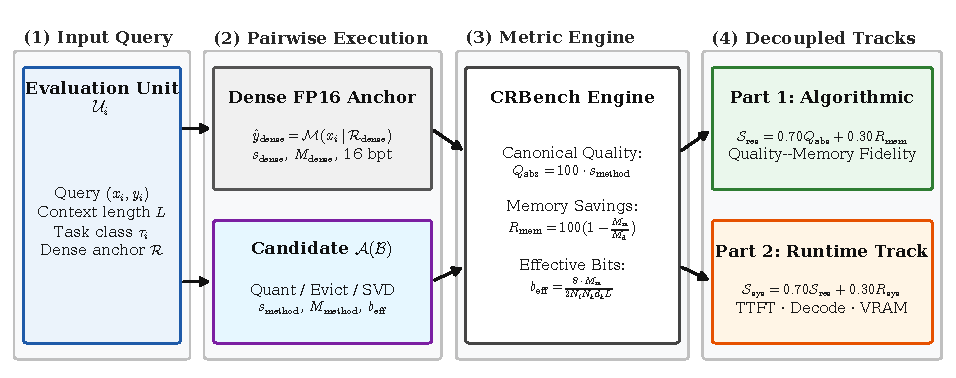
\includegraphics[width=0.94\textwidth]{figures/fig1_framework_overview.pdf}
\caption{\textbf{CRBench Method-Agnostic Evaluation Framework Architecture.} The benchmark decouples evaluation into two complementary tracks: Part~1 (Algorithmic Representation Utility $\mathcal{S}_{\text{res}}$) and Part~2 (Hardware System Track $\mathcal{S}_{\text{sys}}$). Every candidate context representation $\mathcal{A}(\mathcal{B})$ is evaluated pairwise against the base model's uncompressed dense reference $\mathcal{R}_{\text{dense}}$ on the identical input query $(x_i, y_i)$.}
\label{fig:framework_overview}
\end{figure}

\subsection{Limitations of Existing Evaluation Paradigms}
Existing approaches to evaluating long-context models and KV compression techniques suffer from structural shortcomings, summarized in Table~\ref{tab:paradigms}:

\begin{table}[t]
\vspace{6pt}
\centering
\small
\setlength{\tabcolsep}{4.0pt}
\caption{Comparison of Evaluation Paradigms vs. CRBench. Summary of dimensions captured across long-context benchmarks, synthetic needle tests, inference profilers, and CRBench.}
\label{tab:paradigms}
\begin{tabular}{lccccc}
\toprule
\textbf{Evaluation Paradigm} & \textbf{Quality} & \textbf{Memory} & \textbf{Latency} & \textbf{Dense Anchor} & \textbf{Pairwise} \\
\midrule
Long-Context Suites (LongBench, L-Eval) & \cmark & \xmark & \xmark & \xmark & \xmark \\
Synthetic Needle Tests (NIAH, RULER) & \cmark & \xmark & \xmark & \xmark & \xmark \\
Inference Systems Profilers (vLLM) & \xmark & \cmark & \cmark & \xmark & \xmark \\
Ad-hoc Compression Literature & \cmark & $\triangle$ & $\triangle$ & \xmark & \xmark \\
\textbf{CRBench (This Work)} & \textbf{\cmark} & \textbf{\cmark} & \textbf{\cmark} & \textbf{\cmark} & \textbf{\cmark} \\
\bottomrule
\end{tabular}
\end{table}

\begin{enumerate}[leftmargin=*,itemsep=1.5pt]
    \item \textbf{Quality--Resource Disconnection}: Traditional benchmarks (e.g., L-Eval~\citep{an2023leval}, BAMBOO~\citep{dong2023bamboo}, InfiniteBench~\citep{zhang2024infinitebench}) measure accuracy without tracking memory. A method achieving 90\% accuracy while consuming 16 bits per token is treated identically to a method achieving 90\% accuracy at 4 bits per token, despite the latter offering $4\times$ greater hardware efficiency.
    \item \textbf{Cross-Model Confounding}: Absolute task accuracy also reflects the base model's native capability. CRBench therefore reports each model separately and logs paired dense outcomes on the identical query, allowing readers to inspect representation effects without presenting a cross-model score as a causal comparison.
    \item \textbf{Omission of Metadata and Runtime Overheads}: Many compression works report theoretical payload bits while omitting the memory required for scaling factors, outlier vectors, or eviction index tables. Furthermore, algorithms that save memory via uncoalesced memory gathers or CPU--GPU synchronization can severely degrade prefill latency (TTFT) and decode throughput.
\end{enumerate}

% ==============================================================================
% 3. PROBLEM DEFINITION & MATHEMATICAL FORMULATION
% ==============================================================================
\section{Problem Definition \& Mathematical Formulation}
\label{sec:formulation}

\begin{figure}[t]
\centering
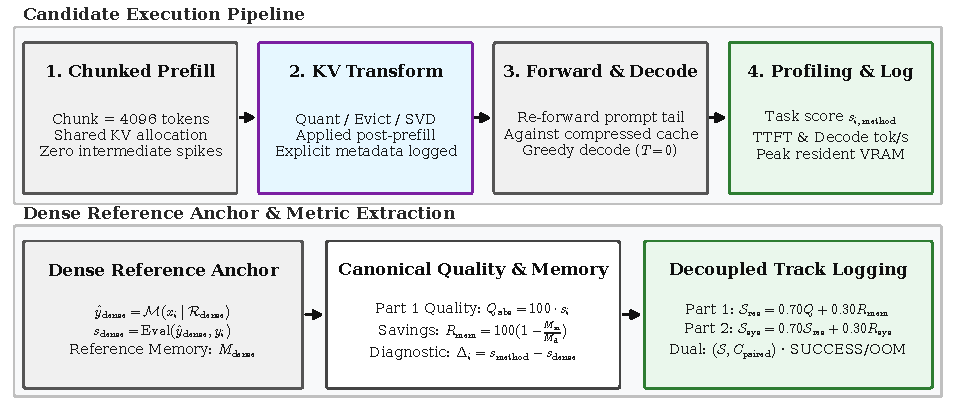
\includegraphics[width=0.94\textwidth]{figures/fig2_query_pipeline.pdf}
\caption{\textbf{Atomic Query-Level Evaluation Pipeline in CRBench.} Execution flow from a single query through chunked prefill, transformed-cache re-forwarding, exact metadata tracking, paired dense diagnostics, canonical quality--memory scoring, and dataset-level aggregation.}
\label{fig:query_pipeline}
\end{figure}

\subsection{The Atomic Evaluation Primitive}
Let $\mathcal{M}$ denote an autoregressive language model parameterized by weights $\Theta$. An evaluation dataset $\mathcal{D} = \{(x_i, y_i, \tau_i, L_i)\}_{i=1}^N$ consists of queries $x_i$, ground-truth target outputs $y_i$, task types $\tau_i$, and prompt context token lengths $L_i$.

Let $\mathcal{A}$ denote a candidate context memory adapter (e.g., INT4 quantization or SnapKV eviction) operating under assigned resource budget $\mathcal{B}$. In standard dense inference, the uncompressed reference adapter is denoted $\mathcal{R}_{\text{dense}}$ (16-bit FP16/BF16 representation).

\begin{definition}[CRBench Atomic Evaluation Unit]
The fundamental evaluation unit in CRBench is the 4-tuple:
\begin{equation}
\label{eq:eval_unit}
\mathcal{U}_i = \Big( \mathcal{M}, \; (x_i, y_i), \; \mathcal{R}_{\text{dense}}, \; \mathcal{A}(\mathcal{B}) \Big)
\end{equation}
For every query $(x_i, y_i)$, CRBench executes:
\begin{enumerate}[leftmargin=*,itemsep=1.0pt]
    \item \textbf{Dense Reference Execution}: Model $\mathcal{M}$ generates prediction $\hat{y}_{i, \text{dense}} = \mathcal{M}(x_i \mid \mathcal{R}_{\text{dense}})$.
    \item \textbf{Candidate Adapter Execution}: Model $\mathcal{M}$ generates prediction $\hat{y}_{i, \text{method}} = \mathcal{M}(x_i \mid \mathcal{A}(\mathcal{B}))$.
    \item \textbf{Quality Measurement}: Raw task scores $s_{i, \text{dense}} = \text{Eval}(\hat{y}_{i, \text{dense}}, y_i) \in [0, 1]$ and $s_{i, \text{method}} = \text{Eval}(\hat{y}_{i, \text{method}}, y_i) \in [0, 1]$ are recorded.
    \item \textbf{Resource Measurement}: Memory footprints $M_{i, \text{dense}}$ and $M_{i, \text{method}}$ (in bytes) are computed analytically and tracked physically.
\end{enumerate}
\end{definition}

\subsection{Canonical Quality and Dense-Reference Diagnostics}
\label{sec:quality}
The canonical leaderboard deliberately uses an absolute task-success quantity. This makes scores comparable across the full suite and keeps a weak dense baseline from inflating a compressed method's apparent retention. The paired dense execution remains essential: it records the reference outcome, enables failure diagnosis, and defines coverage.

\begin{definition}[Canonical Absolute Task Quality]
Let $s_{i,\text{method}} \in [0,1]$ be the task evaluator's score for a completed candidate run. Its canonical quality is:
\begin{equation}
\label{eq:quality_absolute}
Q_{\text{abs},i}=100.0\,\min\left(1.0,\max\left(0.0,s_{i,\text{method}}\right)\right).
\end{equation}
\end{definition}

\paragraph{Paired diagnostics and coverage.} We log the signed paired difference $\Delta_i=s_{i,\text{method}}-s_{i,\text{dense}}$ and report paired execution coverage $C_{\text{paired}}=N_{\text{paired-success}}/N_{\text{total}}$. Thus, a zero score from a completed run is distinguished from an out-of-memory or runtime failure. Relative retention can be recomputed from the logged pairs for a task with a defensible chance floor, but it is not substituted into the canonical reported scores.

\subsection{Memory Resource Accounting (\texorpdfstring{$R_{\text{mem}}$}{R\_mem})}
CRBench enforces explicit state memory accounting. For any adapter $\mathcal{A}$, the total memory consumed by the context representation is partitioned into three additive components:
\begin{equation}
\label{eq:memory_decomposition}
M_{\text{method}}(L) = M_{\text{algo}}(L) + M_{\text{meta}}(L) + M_{\text{align}}(L) \quad [\text{bytes}]
\end{equation}
where $M_{\text{algo}}$ is the raw compressed tensor payload, $M_{\text{meta}}$ represents all mandatory auxiliary metadata (quantization scale factors, zero-point offsets, codebook dictionaries, or 32-bit integer token position index arrays for eviction methods), and $M_{\text{align}}$ represents hardware memory alignment and padding overheads.

\begin{definition}[Effective Bits Per KV Element]
The effective bits-per-element ($b_{\text{eff}}$) measures the total memory footprint normalized by the total uncompressed Key-Value tensor scalar count ($2 \times N_{\text{layers}} \times N_{\text{kv\_heads}} \times d_{\text{head}} \times L$):
\begin{equation}
\label{eq:beff}
b_{\text{eff}} = \frac{8 \cdot M_{\text{method}}(L)}{2 \cdot N_{\text{layers}} \cdot N_{\text{kv\_heads}} \cdot d_{\text{head}} \cdot L} \quad [\text{bits/element}]
\end{equation}
For standard uncompressed 16-bit float KV caches (FP16/BF16), $b_{\text{eff}} = 16.0\,\text{bits/element}$.
\end{definition}

\begin{definition}[Memory Resource Savings]
The normalized memory resource savings $R_{\text{mem}, i} \in [0.0, 100.0]$ is:
\begin{equation}
\label{eq:resource_savings}
R_{\text{mem}, i} = 100.0 \times \max\left(0.0, \; 1.0 - \frac{M_{i, \text{method}}}{M_{i, \text{dense}}}\right)
\end{equation}
\end{definition}

% ==============================================================================
% 4. SCORING FRAMEWORK
% ==============================================================================
\section{CRBench Scoring Formulation}
\label{sec:scoring}

\subsection{Measurement Desiderata for Utility Formulation}
A useful scalar utility must be monotone in both absolute task quality and resource savings, bounded on $[0,100]^2$, and Pareto consistent. The linear utility below satisfies these properties directly; its short proof and a comparison with alternative formulations are deferred to the supplementary material.

\subsection{Part 1: Resource Utility Score (\texorpdfstring{$\mathcal{S}_{\text{res}}$}{S\_res})}
CRBench defines the canonical Part~1 Resource Score using a linear additive utility formulation:
\begin{equation}
\label{eq:part1_score}
\mathcal{S}_{\text{res}, i} = \alpha \cdot Q_{\text{abs},i} + (1 - \alpha) \cdot R_{\text{mem}, i}
\end{equation}
where $\alpha \in [0.10, 0.90]$ is the global quality preference weight, with standard configuration $\alpha = 0.70$.

\paragraph{Default trade-off.} The $\alpha=0.70$ configuration makes a one-point gain in task quality worth $2.33$ points of memory savings. A dense run with perfect task success has score $70.0$, whereas a 4-bit method at $94\%$ task quality and $75\%$ savings has score $88.3$. The sensitivity analysis is supplied in the supplement.

\subsection{Dataset Aggregation \& Coverage Reliability (\texorpdfstring{$C_{\text{paired}}$}{C\_paired})}
For an evaluation dataset $\mathcal{D}$, the aggregate benchmark score is computed by averaging query-level utility scores:
\begin{equation}
\label{eq:dataset_aggregation}
\bar{\mathcal{S}}_{\text{res}} = \frac{1}{|\mathcal{D}|} \sum_{i=1}^{|\mathcal{D}|} \mathcal{S}_{\text{res}, i}, \quad 
\bar{Q}_{\text{abs}} = \frac{1}{|\mathcal{D}|} \sum_{i=1}^{|\mathcal{D}|} Q_{\text{abs},i}, \quad 
\bar{R}_{\text{mem}} = \frac{1}{|\mathcal{D}|} \sum_{i=1}^{|\mathcal{D}|} R_{\text{mem}, i}
\end{equation}
CRBench computes $95\%$ non-parametric bootstrap confidence intervals with $B = 2,000$ resamples.

\paragraph{Coverage Decoupling.} CRBench reports paired query execution coverage $C_{\text{paired}} = \frac{N_{\text{paired\_success}}}{N_{\text{total}}} \in [0.0, 1.0]$ alongside $\mathcal{S}_{\text{res}}$ as a dual-metric pair $(\mathcal{S}_{\text{res}}, C_{\text{paired}})$, rather than multiplicatively folding coverage into $\mathcal{S}_{\text{res}}$. This preserves algorithmic evaluation integrity even if occasional memory allocator faults occur.

% ==============================================================================
% 5. SYSTEM TRACK (PART 2)
% ==============================================================================
\section{System Evaluation Track (Part 2)}
\label{sec:system}

While Part~1 evaluates algorithmic memory representation efficiency, practical deployment requires analyzing physical latency and throughput. An adapter that compresses tensors effectively but relies on un-fused loops or irregular memory gathers can suffer severe latency degradation.

\subsection{Profiled System Metrics}
CRBench incorporates hardware-synchronized wall-clock timers and device memory allocators to capture:
\begin{enumerate}[leftmargin=*,itemsep=1.0pt]
    \item \textbf{Time-To-First-Token ($\text{TTFT}$)}: Total wall-clock time (in seconds) required to process prompt context of length $L$ and emit the first token.
    \item \textbf{Autoregressive Decode Throughput ($\mathcal{T}_{\text{dec}}$)}: Generation speed in tokens per second ($\text{tok/s}$):
    \begin{equation}
    \label{eq:throughput}
    \mathcal{T}_{\text{dec}} = \frac{N_{\text{generated}}}{\Delta t_{\text{decode}}} \quad [\text{tok/s}]
    \end{equation}
    \item \textbf{Peak Resident Device VRAM ($\mathcal{M}_{\text{peak}}$)}: Maximum allocated and reserved GPU memory during inference.
\end{enumerate}

\subsection{System Efficiency and Part 2 Score (\texorpdfstring{$\mathcal{S}_{\text{sys}}$}{S\_sys})}
To evaluate real-world deployment viability under physical hardware constraints, CRBench computes normalized efficiency components relative to the uncompressed dense baseline:
\begin{equation}
\label{eq:relative_efficiency}
\phi_{\text{ttft}} = \min\left(1.0, \; \frac{\text{TTFT}_{\text{dense}}}{\text{TTFT}_{\text{method}}}\right), \quad
\phi_{\text{thru}} = \min\left(1.0, \; \frac{\mathcal{T}_{\text{method}}}{\mathcal{T}_{\text{dense}}}\right), \quad
\phi_{\text{vram}} = \min\left(1.0, \; \frac{\mathcal{M}_{\text{dense}}}{\mathcal{M}_{\text{method}}}\right)
\end{equation}
These three physical dimensions are integrated into a composite hardware efficiency multiplier $\phi \in [0.0, 1.0]$ via a geometric mean:
\begin{equation}
\label{eq:phi_factor}
\phi = \phi_{\text{ttft}}^{0.35} \cdot \phi_{\text{thru}}^{0.35} \cdot \phi_{\text{vram}}^{0.30}, \quad \text{yielding} \quad R_{\text{sys}} = 100.0 \times \phi
\end{equation}
where weights allocate balanced emphasis to interactive responsiveness (TTFT 35\%, decode throughput 35\%) and physical resident device footprint (VRAM 30\%). All system-efficiency components and $\mathcal{S}_{\text{sys}}$ are computed at the individual-query level prior to aggregation; the TTFT, throughput, and VRAM values reported in the tables are descriptive arithmetic means and are not substituted directly into the composite formula.

The composite \textbf{CRBench Part~2 System Serving Score} ($\mathcal{S}_{\text{sys}} \in [0.0, 100.0]$) then combines the algorithmic representation utility ($\mathcal{S}_{\text{res}}$) from Part~1 with physical system efficiency ($R_{\text{sys}}$) using the canonical utility formulation:
\begin{equation}
\label{eq:part2_score}
\mathcal{S}_{\text{sys}} = \alpha \cdot \mathcal{S}_{\text{res}} + (1 - \alpha) \cdot R_{\text{sys}} \quad (\text{with } \alpha = 0.70)
\end{equation}
Methods that meet or exceed the dense baseline on TTFT and decode throughput without exceeding its VRAM footprint achieve $\phi = 1.0$ ($R_{\text{sys}} = 100.0$), while methods incurring prefill stalls or memory bloat receive hardware penalties ($\phi < 1.0$) that rigorously discount their serving score.

% ==============================================================================
% 6. EXPERIMENTAL SETUP
% ==============================================================================
\section{Experimental Setup}
\label{sec:setup}

\subsection{Evaluated Models \& Context Ladders}
We evaluate three open-weight foundation models across 3,150 standardized queries:
\begin{itemize}[leftmargin=*,itemsep=1.0pt]
    \item \textbf{Gemma 4 E2B}: Evaluated across the complete $2\text{K} \to 128\text{K}$ context ladder ($2\text{K}, 8\text{K}, 32\text{K}, 64\text{K}, 128\text{K}$ tokens, 1,050 queries).
    \item \textbf{Gemma 4 E4B}: Evaluated across context horizons from $2\text{K}$ to $32\text{K}$ ($2\text{K}, 4\text{K}, 8\text{K}, 16\text{K}, 32\text{K}$ tokens, 1,050 queries).
    \item \textbf{Qwen2.5 7B}: Evaluated across context horizons from $2\text{K}$ to $32\text{K}$ ($2\text{K}, 4\text{K}, 8\text{K}, 16\text{K}, 32\text{K}$ tokens, 1,050 queries).
\end{itemize}

\subsection{Evaluated Methods}
We evaluate seven representative context compression methods alongside the uncompressed 16-bit dense reference:
\begin{enumerate}[leftmargin=*,itemsep=0.5pt,topsep=1.5pt]
    \item \textbf{KIVI-style INT4 Quantization}: 4-bit asymmetric per-channel keys and 4-bit per-token values following the grouping scheme of KIVI~\citep{liu2024kivi}.
    \item \textbf{SnapKV}: Observation-guided heavy-hitter eviction ($L_{\text{obs}} = 32, k = 7$)~\citep{li2024snapkv}.
    \item \textbf{DKV-Mid / High} (Authors withheld for double-blind review, 2026): Differential KV with 128- / 256-rank subspace and dynamic residuals.
    \item \textbf{Low-Rank KV}: Per-head mean-centered truncated SVD projection~\citep{sharma2023truth}.
    \item \textbf{StreamingLLM}: Attention sink ($N_{\text{sink}} = 4$) + rolling local window eviction~\citep{xiao2023streamingllm}.
    \item \textbf{KV-Merging}: Temporal adjacent token mean-pooling~\citep{ge2023model}.
    \item \textbf{Dense FP16}: Full uncompressed 16-bit reference baseline ($b_{\text{eff}} = 16.0$ bpt).
\end{enumerate}

\subsection{Evaluation Tasks}
\begin{enumerate}[leftmargin=*,itemsep=0.5pt,topsep=1.5pt]
    \item \textbf{Single \& Multi NIAH}: Single- and distributed multi-target needle retrieval at parameterized insertion depths.
    \item \textbf{RULER KV}: High-entropy dictionary key-value lookup amid distracting pairs~\citep{hsieh2024ruler}.
    \item \textbf{Variable Tracking}: Multi-step variable reassignment tracking~\citep{hsieh2024ruler}.
    \item \textbf{Multi-Hop QA}: Cross-document synthetic multi-hop reasoning.
\end{enumerate}

% ==============================================================================
% 7. RESULTS
% ==============================================================================
\section{Results}
\label{sec:results}

\subsection{Cross-Model Algorithmic Representation Fidelity (\texorpdfstring{$\mathcal{S}_{\text{res}}$}{S\_res})}

Table~\ref{tab:sres_cross} presents the Part~1 leaderboard across all three models under canonical scoring $\mathcal{S}_{\text{res}} = 0.70 \cdot Q_{\text{abs}} + 0.30 \cdot R_{\text{mem}}^{\text{agg}}$.

\begin{table}[t]
\vspace{6pt}
\centering
\small
\caption{\textbf{Cross-Model Part 1 ($\mathcal{S}_{\text{res}}$) Leaderboard.} Evaluated under canonical Option~B physical memory aggregation across 3,150 queries. Best score per model in \textbf{bold}.}
\label{tab:sres_cross}
\resizebox{\textwidth}{!}{%
\begin{tabular}{l ccc ccc ccc}
\toprule
& \multicolumn{3}{c}{\textbf{Gemma 4 E2B (2K--128K)}} & \multicolumn{3}{c}{\textbf{Gemma 4 E4B (2K--32K)}} & \multicolumn{3}{c}{\textbf{Qwen2.5 7B (2K--32K)}} \\
\cmidrule(lr){2-4}\cmidrule(lr){5-7}\cmidrule(lr){8-10}
\textbf{Method} & \textbf{Accuracy} & $b_{\text{eff}}^{\text{agg}}$ & $\mathcal{S}_{\text{res}}$ & \textbf{Accuracy} & $b_{\text{eff}}^{\text{agg}}$ & $\mathcal{S}_{\text{res}}$ & \textbf{Accuracy} & $b_{\text{eff}}^{\text{agg}}$ & $\mathcal{S}_{\text{res}}$ \\
\midrule
\textbf{KIVI (INT4)}         & 46.4\% & 6.01 bpt & 51.2 & 62.0\% & 6.04 bpt & \textbf{62.1} & 60.7\% & 6.04 bpt & \textbf{61.1} \\
\textbf{SnapKV}              & 46.8\% & 6.00 bpt & \textbf{51.5} & 60.0\% & 6.00 bpt & 60.8 & 58.2\% & 6.00 bpt & 59.5 \\
\textbf{DKV-Mid}             & 44.7\% & 5.46 bpt & 51.0 & 55.3\% & 5.00 bpt & 59.4 & 53.3\% & 5.84 bpt & 56.3 \\
\textbf{DKV-High}            & 46.7\% & 10.78 bpt & 42.5 & 61.3\% & 10.68 bpt & 52.9 & 59.1\% & 12.14 bpt & 48.6 \\
\textbf{Dense FP16}          & 46.4\% & 16.00 bpt & 32.5 & 64.0\% & 16.00 bpt & 44.8 & 60.0\% & 16.00 bpt & 42.0 \\
\textbf{Low-Rank KV}         & 31.2\% & 6.07 bpt & 40.5 & 48.8\% & 6.27 bpt & 52.4 & 28.6\% & 6.09 bpt & 38.6 \\
\textbf{StreamingLLM}        & 22.9\% & 6.00 bpt & 34.8 & 25.5\% & 6.00 bpt & 36.6 & 36.5\% & 6.00 bpt & 44.3 \\
\textbf{KV-Merging}          & 13.3\% & 6.01 bpt & 28.0 & 25.3\% & 6.03 bpt & 36.4 & 19.9\% & 6.03 bpt & 32.6 \\
\bottomrule
\end{tabular}%
}
\end{table}

\begin{figure}[t]
\centering
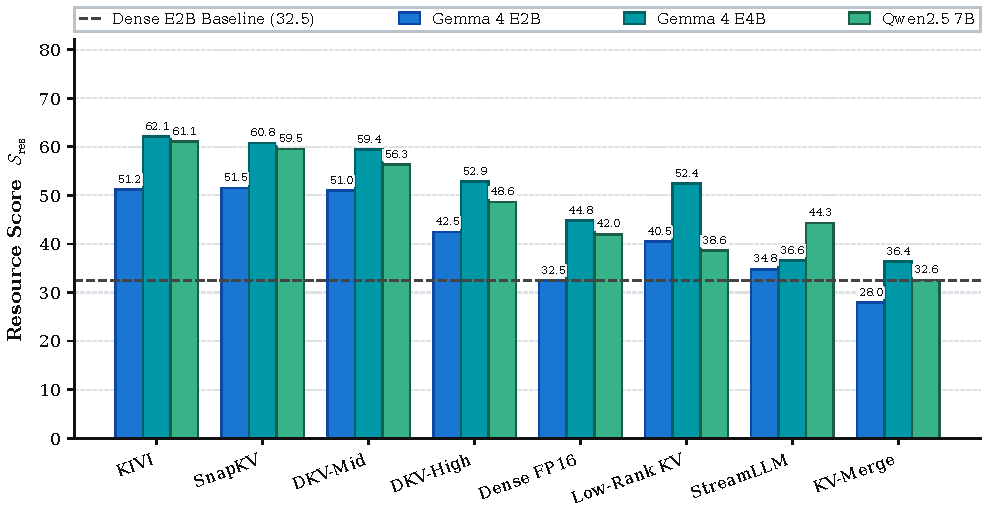
\includegraphics[width=0.94\textwidth]{figures/fig3_sres_cross.pdf}
\caption{\textbf{Cross-Model Part~1 Resource Utility ($\mathcal{S}_{\text{res}}$) Comparison.} Evaluated across Gemma~4 E2B, Gemma~4 E4B, and Qwen2.5~7B.}
\label{fig:sres_cross}
\end{figure}

\subsection{Cross-Model Hardware System Serving Utility (\texorpdfstring{$\mathcal{S}_{\text{sys}}$}{S\_sys})}

Table~\ref{tab:ssys_cross} presents the Part~2 system scores. The per-model distribution is provided in the supplementary material.

\begin{table}[h]
\vspace{6pt}
\centering
\small
\setlength{\tabcolsep}{5pt}
\caption{\textbf{Cross-Model Part 2 Hardware System Serving Utility ($\mathcal{S}_{\text{sys}}$).} Ranked by cross-model mean score.}
\label{tab:ssys_cross}
\begin{tabular}{lcccc}
\toprule
\textbf{Method} & \textbf{Gemma 4 E2B} & \textbf{Gemma 4 E4B} & \textbf{Qwen2.5 7B} & \textbf{Cross-Model Mean $\mathcal{S}_{\text{sys}}$} \\
\midrule
\textbf{KIVI (INT4)}         & 64.6 & 73.4 & 72.8 & \textbf{70.3} \\
\textbf{DKV-Mid}             & 59.1 & 66.3 & 54.2 & \textbf{59.9} \\
\textbf{Low-Rank KV}         & 57.4 & 65.9 & 54.9 & \textbf{59.4} \\
\textbf{Dense FP16}          & 52.8 & 61.4 & 59.4 & \textbf{57.8} \\
\textbf{StreamingLLM}        & 54.3 & 55.6 & 61.0 & \textbf{57.0} \\
\textbf{SnapKV}              & 60.6 & 48.6 & 53.7 & \textbf{54.3} \\
\textbf{DKV-High}            & 52.7 & 60.0 & 48.5 & \textbf{53.7} \\
\textbf{KV-Merging}          & 49.6 & 55.5 & 52.8 & \textbf{52.6} \\
\bottomrule
\end{tabular}
\end{table}

\subsection{Task-Wise Performance Breakdown}

Figure~\ref{fig:task_heatmap} visualizes the cross-model mean accuracy by task archetype.

\begin{figure}[t]
\centering
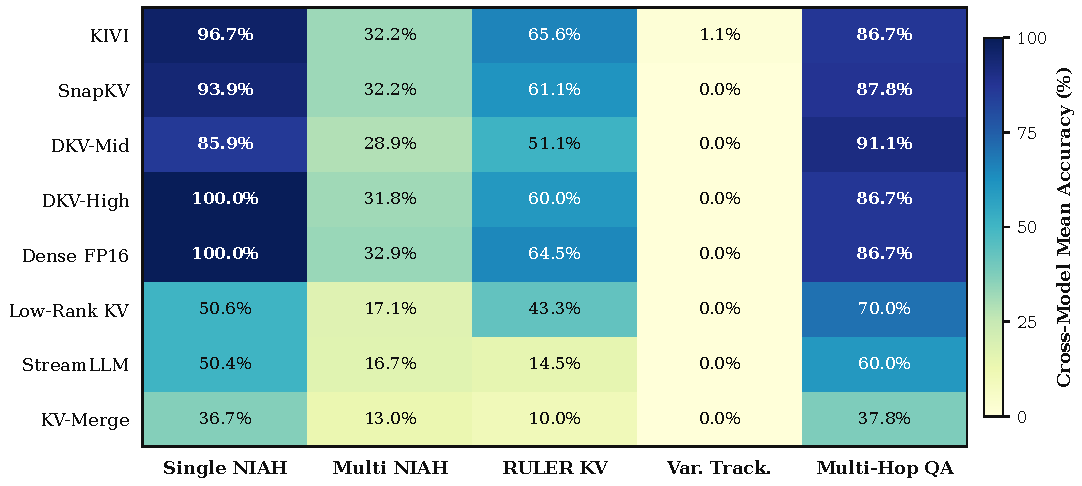
\includegraphics[width=0.82\textwidth]{figures/fig5_task_heatmap.pdf}
\caption{\textbf{Task-Wise Accuracy Heatmap Across Compression Paradigms.} Cross-model average accuracy (\%) across all three evaluated models.}
\label{fig:task_heatmap}
\end{figure}

\subsection{Ultra-Long Context Ladder (\texorpdfstring{$2\text{K} \to 128\text{K}$}{2K to 128K}) Scaling}

Figure~\ref{fig:context_scaling} traces performance across the full 2K--128K context ladder on Gemma~4 E2B, illustrating the degradation cliff beyond 64K tokens.

\begin{figure}[t]
\centering
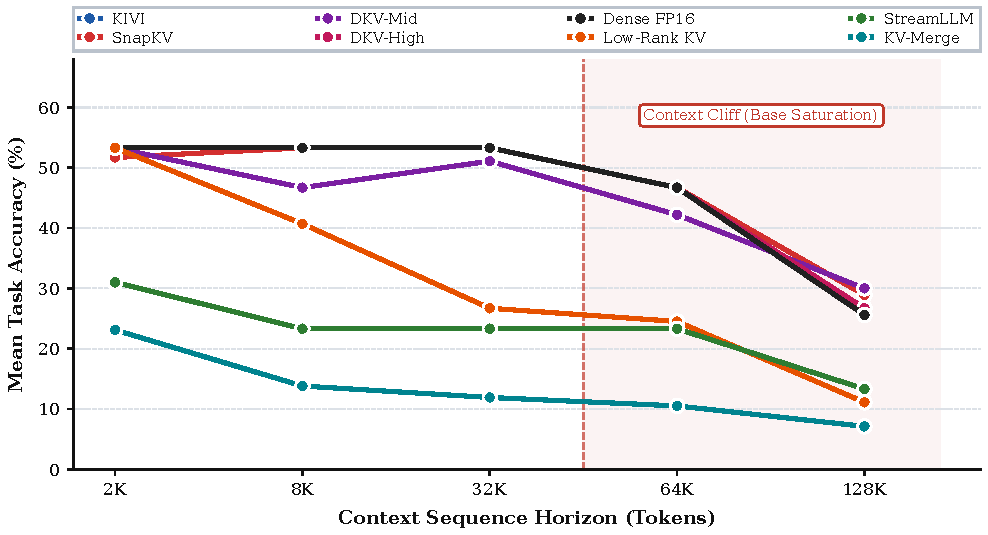
\includegraphics[width=0.88\textwidth]{figures/fig6_context_scaling.pdf}
\caption{\textbf{Ultra-Long Context Ladder Scaling (2K to 128K Tokens) on Gemma 4 E2B.} Accuracy averaged across all 5 tasks, showing sharp degradation at 64K--128K shared with the uncompressed baseline.}
\label{fig:context_scaling}
\end{figure}

\subsection{Empirical Quality--Memory Pareto Frontier}

Figure~\ref{fig:pareto_frontier} maps task accuracy against effective bits-per-element $b_{\text{eff}}$, highlighting the non-dominated Pareto frontier across all three models.

\begin{figure}[t]
\centering
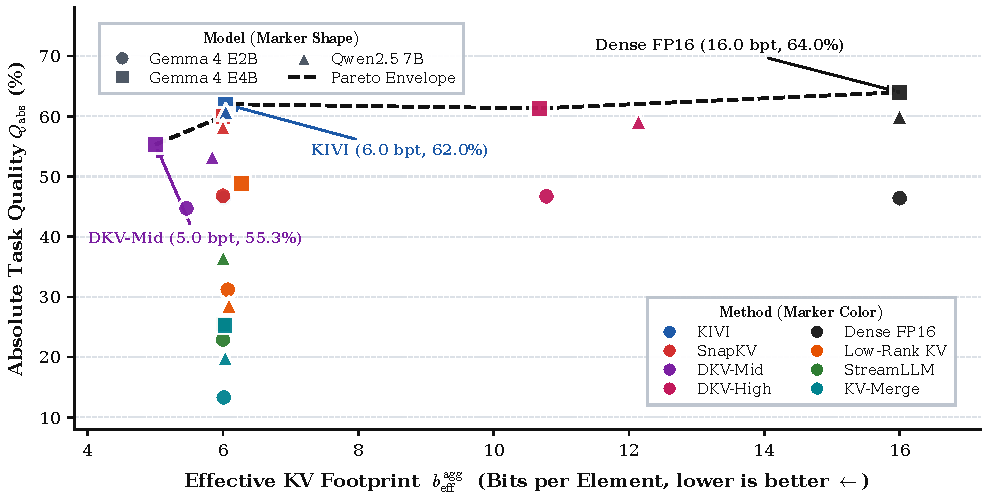
\includegraphics[width=0.88\textwidth]{figures/fig7_pareto_frontier.pdf}
\caption{\textbf{Quality--Memory Pareto Frontier Across 3 Foundation Models.} Evaluated across 24 configurations, mapping task accuracy against effective bits-per-element $b_{\text{eff}}$. Marker shapes denote foundation model (circle: Gemma~4 E2B, square: Gemma~4 E4B, triangle: Qwen2.5~7B); marker colors denote compression method.}
\label{fig:pareto_frontier}
\end{figure}

% ==============================================================================
% 8. DISCUSSION
% ==============================================================================
% ==============================================================================
% 8. DISCUSSION
% ==============================================================================
\section{Analysis \& Discussion}
\label{sec:discussion}

\paragraph{KIVI Dominates System Serving ($\bar{\mathcal{S}}_{\text{sys}} = 70.3$).}
KIVI-style INT4 quantization achieves the highest cross-model system score because asymmetric quantization operates during cache writes without prefill latency spikes, maintaining $\phi \ge 0.96\times$ across all models.

\paragraph{SnapKV's Prefill Hardware Penalty.}
While SnapKV attains high algorithmic utility ($\mathcal{S}_{\text{res}} = 60.8$ on E4B), un-fused observation pooling on 32K sequences inflates TTFT to $83.4$s and peak VRAM to 2,632 MB ($\phi = 0.20\times$), dropping its Part~2 score to $48.6$ and confirming the necessity of decoupled system profiling.

\paragraph{DKV-Mid Pushes the Memory Frontier ($5.00$--$5.84$ bpt).}
DKV-Mid operates at low bitrates ($5.00$ bpt on E4B) and attains the highest cross-model Multi-Hop QA accuracy in our evaluated suite ($91.1\%$). However, SVD projection increases TTFT ($22.3$s on E2B, $39.6$s on 7B), resulting in $\phi \approx 0.49$--$0.83\times$.

\paragraph{Variable Tracking: Model-Level Limitation.} All evaluated methods, including uncompressed dense FP16, score near $0.0\%$ on Variable Tracking, indicating that the evaluated models have a substantial capability limitation on this task that is not explained by KV compression alone.

% ==============================================================================
% 9. LIMITATIONS
% ==============================================================================
\section{Limitations \& Research Scope}
\label{sec:limitations}
We identify four key operational boundaries: (1)~\textbf{Model Scale}: Current evaluation benchmarks 2B to 7B architectures; future extensions will evaluate 13B+ and 70B+ model families. (2)~\textbf{Task Coverage}: Our suite prioritizes long-context needle retrieval, associative lookup, and multi-hop reasoning; open-ended agentic dialogues and summarization represent natural next steps. (3)~\textbf{Hardware Scope}: Profiling is conducted on single-node workstation GPUs; distributed multi-GPU serving may alter Part~2 communication costs. (4)~\textbf{Kernel Fusion}: Algorithms evaluated via pure PyTorch incur prefill memory and dispatch latency penalties that dedicated fused CUDA/Triton kernels can substantially mitigate.

% ==============================================================================
% 10. CONCLUSION
% ==============================================================================
\section{Conclusion}
\label{sec:conclusion}
We presented \textbf{CRBench}, a method-agnostic, resource-aware evaluation framework for long-context LLMs. By anchoring evaluations pairwise against the uncompressed dense reference, enforcing explicit memory accounting via $b_{\text{eff}}$, and decoupling algorithmic utility ($\mathcal{S}_{\text{res}}$) from hardware serving ($\mathcal{S}_{\text{sys}}$), CRBench establishes a rigorous foundation for evaluating context memory representations.

% ==============================================================================
% BROADER IMPACT STATEMENT
% ==============================================================================
\subsubsection*{Broader Impact Statement}
\label{sec:broader_impact}
Context representation and compression technologies directly influence the economic accessibility and environmental footprint of frontier artificial intelligence. By reducing KV cache memory demands by up to $3.2\times$, efficient context representations democratize long-context serving on commodity hardware and substantially decrease data center energy consumption and carbon emissions. However, aggressive eviction and lossy quantization can induce behavioral drift, hallucinations, or silent omission of needle facts in high-stakes domains (e.g., clinical retrieval or legal contract analysis). CRBench directly mitigates these risks by providing an auditable, multi-dimensional evaluation suite that rigorously exposes failure modes and hardware bottlenecks before compression algorithms are deployed in production systems.

% ==============================================================================
% REFERENCES
% ==============================================================================
\bibliographystyle{plainnat}
\begingroup
\small
\begin{thebibliography}{24}


\bibitem[Achiam et~al.(2023)]{achiam2023gpt4} Achiam, J., Adler, S., Agarwal, S., et~al. (2023). GPT-4 technical report. \textit{arXiv preprint arXiv:2303.08774}.

\bibitem[An et~al.(2023)]{an2023leval} An, C., Gong, S., Zhong, M., et~al. (2023). L-Eval: Instituting standardized evaluation for long context language models. \textit{arXiv preprint arXiv:2307.11088}.

\bibitem[Bai et~al.(2023a)]{bai2023qwen} Bai, J., Bai, S., Chu, Y., et~al. (2023a). Qwen technical report. \textit{arXiv preprint arXiv:2309.16609}.

\bibitem[Bai et~al.(2023b)]{bai2023longbench} Bai, Y., Lv, X., Zhang, J., et~al. (2023b). LongBench: A bilingual, multitask benchmark for long context understanding. \textit{arXiv preprint arXiv:2308.14508}.

\bibitem[Bai et~al.(2024)]{bai2024longbenchv2} Bai, Y., Lv, X., Zhang, J., et~al. (2024). LongBench v2: Towards deeper understanding of long context large language models. \textit{arXiv preprint arXiv:2412.15204}.

\bibitem[Brown et~al.(2020)]{brown2020language} Brown, T., Mann, B., Ryder, N., et~al. (2020). Language models are few-shot learners. In \textit{NeurIPS}, vol.~33, pp. 1877--1901.

\bibitem[Authors withheld for double-blind review(2026)]{chimurkar2026dkv} [Authors withheld for double-blind review] (2026). DKV: Anchor + Low-Rank Differential KV-Cache Compression for Scalable Long-Context Inference. \textit{Preprint under double-blind review}.

\bibitem[DeepSeek-AI(2024)]{deepseek2024v2} DeepSeek-AI (2024). DeepSeek-V2: A strong, economical, and efficient Mixture-of-Experts language model. \textit{arXiv preprint arXiv:2405.04434}.

\bibitem[Dettmers et~al.(2022)]{dettmers2022llmint8} Dettmers, T., Lewis, M., Belkada, Y., and Zettlemoyer, L. (2022). LLM.int8(): 8-bit matrix multiplication for transformers at scale. In \textit{NeurIPS}, vol.~35, pp. 30318--30332.

\bibitem[Dong et~al.(2023)]{dong2023bamboo} Dong, Z., Tang, T., Dai, J., et~al. (2023). BAMBOO: A comprehensive benchmark for evaluating long-sequence language models. \textit{arXiv preprint arXiv:2309.13345}.

\bibitem[Ge et~al.(2023)]{ge2023model} Ge, S., Zhang, Y., Liu, L., et~al. (2023). Model tells you what to discard: Adaptive KV cache compression for LLMs. \textit{arXiv preprint arXiv:2310.01801}.

\bibitem[Hooper et~al.(2024)]{hooper2024kvquant} Hooper, C., Kim, S., Mohammadzadeh, H., et~al. (2024). KVQuant: Towards 10 million context length LLM inference with KV cache quantization. In \textit{NeurIPS}.

\bibitem[Hsieh et~al.(2024)]{hsieh2024ruler} Hsieh, C.-Y., Sun, S., Kriman, S., et~al. (2024). RULER: What's the real context size of your long-context language model? \textit{arXiv preprint arXiv:2404.06654}.

\bibitem[Kamradt(2023)]{kamradt2023needle} Kamradt, G. (2023). Needle in a haystack - pressure testing LLMs. \textit{GitHub repository: gkamradt/LLMTest\_NeedleInAHaystack}.

\bibitem[Li et~al.(2024)]{li2024snapkv} Li, Y., Huang, Y., Yang, B., et~al. (2024). SnapKV: LLM knows what you are looking for before generation. In \textit{NeurIPS}.

\bibitem[Liu et~al.(2023)]{liu2023scissorhands} Liu, Z., Desai, A., Liao, F., et~al. (2023). Scissorhands: Exploiting the persistence of importance in LLM KV cache. In \textit{NeurIPS}.

\bibitem[Liu et~al.(2024)]{liu2024kivi} Liu, Z., Yuan, J., Jin, H., et~al. (2024). KIVI: A tuning-free asymmetric 2bit quantization for KV cache. In \textit{ICML}.

\bibitem[Reid et~al.(2024)]{reid2024gemini} Reid, M., Savinov, N., Teplyashin, D., et~al. (2024). Gemini 1.5: Unlocking multimodal understanding across millions of tokens of context. \textit{arXiv preprint arXiv:2403.05530}.

\bibitem[Sharma et~al.(2024)]{sharma2023truth} Sharma, P., Ash, J.~T., and Misra, D. (2024). The truth is in there: Improving reasoning in language models with layer-selective rank reduction. In \textit{ICLR}.

\bibitem[Touvron et~al.(2023)]{touvron2023llama} Touvron, H., Lavril, T., Izacard, G., et~al. (2023). LLaMA: Open and efficient foundation language models. \textit{arXiv preprint arXiv:2302.13971}.

\bibitem[Vaswani et~al.(2017)]{vaswani2017attention} Vaswani, A., Shazeer, N., Parmar, N., et~al. (2017). Attention is all you need. In \textit{NeurIPS}, vol.~30, pp. 5998--6008.

\bibitem[Xiao et~al.(2023)]{xiao2023streamingllm} Xiao, G., Tian, Y., Chen, B., et~al. (2023). Efficient streaming language models with attention sinks. In \textit{ICLR}.

\bibitem[Zhang et~al.(2023)]{zhang2023h2o} Zhang, Z., Sheng, Y., Zheng, T., et~al. (2023). $\text{H}_2\text{O}$: Heavy-hitter oracle for efficient generative inference of large language models. In \textit{NeurIPS}.

\bibitem[Zhang et~al.(2024a)]{zhang2024pyramidkv} Zhang, Y., Du, X., Liu, C., et~al. (2024a). PyramidKV: Dynamic KV cache compression based on pyramid information funneling. \textit{arXiv preprint arXiv:2406.02069}.

\bibitem[Zhang et~al.(2024b)]{zhang2024infinitebench} Zhang, X., Chen, Y., Hu, S., et~al. (2024b). $\infty$-Bench: Extending context window to 100K+ for comprehensive evaluation of LLMs. In \textit{ACL}.

\end{thebibliography}
\endgroup


\clearpage
\appendix

% ==============================================================================
% SECTION A: FULL PER-MODEL LEADERBOARDS
% ==============================================================================
\section{Full Per-Model Leaderboards}
\label{sec:app_leaderboards}

This section provides complete Part~1 (Algorithmic Representation Fidelity $\mathcal{S}_{\text{res}}$) and Part~2 (Hardware System Serving Utility $\mathcal{S}_{\text{sys}}$) leaderboards for all three evaluated foundation model families across 3,150 queries.

\subsection{Gemma 4 E2B Leaderboard (\texorpdfstring{$2\text{K} \to 128\text{K}$}{2K to 128K} Context Ladder, 1,050 Queries)}

\begin{table}[h]
\vspace{6pt}
\centering
\small
\caption{Gemma 4 E2B Part 1 ($\mathcal{S}_{\text{res}}$) Algorithmic Representation Leaderboard.}
\label{tab:e2b_sres}
\begin{tabular}{clcccc}
\toprule
\textbf{Rank} & \textbf{Method} & \textbf{Accuracy} & $b_{\text{eff}}^{\text{agg}}$ & \textbf{VRAM Saved} & $\mathcal{S}_{\text{res}}$ \\
\midrule
1 & \textbf{SnapKV} & 46.8\% & 6.00 bpt & 62.5\% & \textbf{51.5} \\
2 & \textbf{KIVI} & 46.4\% & 6.01 bpt & 62.4\% & 51.2 \\
3 & \textbf{DKV-Mid} & 44.7\% & 5.46 bpt & 65.9\% & 51.0 \\
4 & \textbf{DKV-High} & 46.7\% & 10.78 bpt & 32.6\% & 42.5 \\
5 & \textbf{Low-Rank KV} & 31.2\% & 6.07 bpt & 62.1\% & 40.5 \\
6 & \textbf{StreamingLLM} & 22.9\% & 6.00 bpt & 62.5\% & 34.8 \\
7 & \textbf{Dense FP16} (Reference) & 46.4\% & 16.00 bpt & 0.0\% & 32.5 \\
8 & \textbf{KV-Merging} & 13.3\% & 6.01 bpt & 62.5\% & 28.0 \\
\bottomrule
\end{tabular}
\end{table}

\begin{table}[h]
\vspace{6pt}
\centering
\small
\caption{Gemma 4 E2B Part 2 ($\mathcal{S}_{\text{sys}}$) Hardware System Serving Leaderboard.}
\label{tab:e2b_ssys}
\begin{tabular}{clccccccc}
\toprule
\textbf{Rank} & \textbf{Method} & $\mathcal{S}_{\text{sys}}$ & $\mathcal{S}_{\text{res}}$ & \textbf{TTFT} & \textbf{Decode} & \textbf{Peak VRAM} & $\phi$ \\
\midrule
1 & \textbf{KIVI} & \textbf{64.6} & 51.2 & 12.51s & 11.9 tok/s & 847.0 MB & 0.96$\times$ \\
2 & \textbf{SnapKV} & 60.6 & 51.5 & 13.04s & 12.9 tok/s & 2088.2 MB & 0.82$\times$ \\
3 & \textbf{DKV-Mid} & 59.1 & 51.0 & 22.26s & 13.8 tok/s & 1389.9 MB & 0.78$\times$ \\
4 & \textbf{Low-Rank KV} & 57.4 & 40.5 & 12.80s & 12.3 tok/s & 849.8 MB & 0.97$\times$ \\
5 & \textbf{StreamingLLM} & 54.3 & 34.8 & 12.58s & 13.7 tok/s & 847.4 MB & 1.00$\times$ \\
6 & \textbf{Dense FP16} & 52.8 & 32.5 & 13.18s & 13.4 tok/s & 1118.4 MB & 1.00$\times$ \\
7 & \textbf{DKV-High} & 52.7 & 42.5 & 23.40s & 13.8 tok/s & 1391.0 MB & 0.77$\times$ \\
8 & \textbf{KV-Merging} & 49.6 & 28.0 & 12.59s & 13.7 tok/s & 847.8 MB & 1.00$\times$ \\
\bottomrule
\end{tabular}
\end{table}

\clearpage
\subsection{Gemma 4 E4B Leaderboard (\texorpdfstring{$2\text{K} \to 32\text{K}$}{2K to 32K} Context Ladder, 1,050 Queries)}

\begin{table}[h]
\vspace{6pt}
\centering
\small
\caption{Gemma 4 E4B Part 1 ($\mathcal{S}_{\text{res}}$) Algorithmic Representation Leaderboard.}
\label{tab:e4b_sres}
\begin{tabular}{clcccc}
\toprule
\textbf{Rank} & \textbf{Method} & \textbf{Accuracy} & $b_{\text{eff}}^{\text{agg}}$ & \textbf{VRAM Saved} & $\mathcal{S}_{\text{res}}$ \\
\midrule
1 & \textbf{KIVI} & 62.0\% & 6.04 bpt & 62.2\% & \textbf{62.1} \\
2 & \textbf{SnapKV} & 60.0\% & 6.00 bpt & 62.5\% & 60.8 \\
3 & \textbf{DKV-Mid} & 55.3\% & 5.00 bpt & 68.7\% & 59.4 \\
4 & \textbf{DKV-High} & 61.3\% & 10.68 bpt & 33.3\% & 52.9 \\
5 & \textbf{Low-Rank KV} & 48.8\% & 6.27 bpt & 60.8\% & 52.4 \\
6 & \textbf{Dense FP16} (Reference) & 64.0\% & 16.00 bpt & 0.0\% & 44.8 \\
7 & \textbf{StreamingLLM} & 25.5\% & 6.00 bpt & 62.5\% & 36.6 \\
8 & \textbf{KV-Merging} & 25.3\% & 6.03 bpt & 62.3\% & 36.4 \\
\bottomrule
\end{tabular}
\end{table}

\begin{table}[h]
\vspace{6pt}
\centering
\small
\caption{Gemma 4 E4B Part 2 ($\mathcal{S}_{\text{sys}}$) Hardware System Serving Leaderboard.}
\label{tab:e4b_ssys}
\begin{tabular}{clccccccc}
\toprule
\textbf{Rank} & \textbf{Method} & $\mathcal{S}_{\text{sys}}$ & $\mathcal{S}_{\text{res}}$ & \textbf{TTFT} & \textbf{Decode} & \textbf{Peak VRAM} & $\phi$ \\
\midrule
1 & \textbf{KIVI} & \textbf{73.4} & 62.1 & 2.84s & 12.8 tok/s & 761.3 MB & 1.00$\times$ \\
2 & \textbf{DKV-Mid} & 66.3 & 59.4 & 5.06s & 12.3 tok/s & 760.7 MB & 0.83$\times$ \\
3 & \textbf{Low-Rank KV} & 65.9 & 52.4 & 3.18s & 13.1 tok/s & 761.5 MB & 0.97$\times$ \\
4 & \textbf{Dense FP16} & 61.4 & 44.8 & 2.96s & 12.4 tok/s & 761.5 MB & 1.00$\times$ \\
5 & \textbf{DKV-High} & 60.0 & 52.9 & 6.25s & 12.2 tok/s & 761.0 MB & 0.76$\times$ \\
6 & \textbf{StreamingLLM} & 55.6 & 36.6 & 2.92s & 13.6 tok/s & 761.4 MB & 1.00$\times$ \\
7 & \textbf{KV-Merging} & 55.5 & 36.4 & 2.91s & 13.5 tok/s & 761.5 MB & 1.00$\times$ \\
8 & \textbf{SnapKV} & 48.6 & 60.8 & 83.38s & 10.6 tok/s & 2632.4 MB & 0.20$\times$ \\
\bottomrule
\end{tabular}
\end{table}

\clearpage
\subsection{Qwen2.5 7B Leaderboard (\texorpdfstring{$2\text{K} \to 32\text{K}$}{2K to 32K} Context Ladder, 1,050 Queries)}

\begin{table}[h]
\vspace{6pt}
\centering
\small
\caption{Qwen2.5 7B Part 1 ($\mathcal{S}_{\text{res}}$) Algorithmic Representation Leaderboard.}
\label{tab:q7b_sres}
\begin{tabular}{clcccc}
\toprule
\textbf{Rank} & \textbf{Method} & \textbf{Accuracy} & $b_{\text{eff}}^{\text{agg}}$ & \textbf{VRAM Saved} & $\mathcal{S}_{\text{res}}$ \\
\midrule
1 & \textbf{KV-Quant} & 60.7\% & 6.04 bpt & 62.2\% & \textbf{61.1} \\
2 & \textbf{SnapKV} & 58.2\% & 6.00 bpt & 62.5\% & 59.5 \\
3 & \textbf{DKV-Mid} & 53.3\% & 5.84 bpt & 63.5\% & 56.3 \\
4 & \textbf{DKV-High} & 59.1\% & 12.14 bpt & 24.1\% & 48.6 \\
5 & \textbf{StreamingLLM} & 36.5\% & 6.00 bpt & 62.5\% & 44.3 \\
6 & \textbf{Dense FP16} (Reference) & 60.0\% & 16.00 bpt & 0.0\% & 42.0 \\
7 & \textbf{Low-Rank KV} & 28.6\% & 6.09 bpt & 62.0\% & 38.6 \\
8 & \textbf{KV-Merging} & 19.9\% & 6.03 bpt & 62.3\% & 32.6 \\
\bottomrule
\end{tabular}
\end{table}

\begin{table}[h]
\vspace{6pt}
\centering
\small
\caption{Qwen2.5 7B Part 2 ($\mathcal{S}_{\text{sys}}$) Hardware System Serving Leaderboard.}
\label{tab:q7b_ssys}
\begin{tabular}{clccccccc}
\toprule
\textbf{Rank} & \textbf{Method} & $\mathcal{S}_{\text{sys}}$ & $\mathcal{S}_{\text{res}}$ & \textbf{TTFT} & \textbf{Decode} & \textbf{Peak VRAM} & $\phi$ \\
\midrule
1 & \textbf{KV-Quant} & \textbf{72.8} & 61.1 & 5.46s & 16.4 tok/s & 3854.3 MB & 1.00$\times$ \\
2 & \textbf{StreamingLLM} & 61.0 & 44.3 & 5.51s & 24.9 tok/s & 3854.4 MB & 1.00$\times$ \\
3 & \textbf{Dense FP16} & 59.4 & 42.0 & 5.56s & 16.3 tok/s & 3854.2 MB & 1.00$\times$ \\
4 & \textbf{Low-Rank KV} & 54.9 & 38.6 & 6.82s & 18.1 tok/s & 3854.4 MB & 0.93$\times$ \\
5 & \textbf{DKV-Mid} & 54.2 & 56.3 & 39.55s & 15.3 tok/s & 3854.2 MB & 0.49$\times$ \\
6 & \textbf{SnapKV} & 53.7 & 59.5 & 58.69s & 22.2 tok/s & 5132.6 MB & 0.40$\times$ \\
7 & \textbf{KV-Merging} & 52.8 & 32.6 & 5.51s & 25.8 tok/s & 3854.4 MB & 1.00$\times$ \\
8 & \textbf{DKV-High} & 48.5 & 48.6 & 41.88s & 15.3 tok/s & 3854.5 MB & 0.48$\times$ \\
\bottomrule
\end{tabular}
\end{table}

\clearpage
% ==============================================================================
% SECTION B: FULL TASK-WISE BREAKDOWN TABLES
% ==============================================================================
\section{Full Task-Wise Breakdown Tables}
\label{sec:app_tasks}

\subsection{Gemma 4 E2B Task Breakdown (5 Tasks \texorpdfstring{$\times$}{x} 5 Context Lengths)}

\begin{table}[h]
\vspace{6pt}
\centering
\small
\caption{Gemma 4 E2B Task-Wise Accuracy Breakdown across Context Lengths (2K to 128K tokens).}
\label{tab:e2b_task_breakdown}
\begin{tabular}{lcccccc}
\toprule
\textbf{Task / Method} & \textbf{2K} & \textbf{8K} & \textbf{32K} & \textbf{64K} & \textbf{128K} & \textbf{Mean Acc} \\
\midrule
\multicolumn{7}{l}{\textbf{Task 1: Single Needle in a Haystack (Single NIAH)}} \\
\textbf{KIVI} & 100.0\% & 100.0\% & 100.0\% & 100.0\% & 100.0\% & \textbf{100.0\%} \\
\textbf{DKV-High} & 100.0\% & 100.0\% & 100.0\% & 100.0\% & 100.0\% & \textbf{100.0\%} \\
\textbf{Dense FP16} & 100.0\% & 100.0\% & 100.0\% & 100.0\% & 100.0\% & \textbf{100.0\%} \\
\textbf{SnapKV} & 91.7\% & 100.0\% & 100.0\% & 100.0\% & 100.0\% & 98.3\% \\
\textbf{DKV-Mid} & 100.0\% & 100.0\% & 100.0\% & 100.0\% & 83.3\% & 96.7\% \\
\textbf{Low-Rank KV} & 100.0\% & 53.3\% & 50.0\% & 50.0\% & 50.0\% & 60.7\% \\
\textbf{StreamingLLM} & 54.9\% & 50.0\% & 50.0\% & 50.0\% & 50.0\% & 51.0\% \\
\textbf{KV-Merging} & 48.7\% & 52.1\% & 42.7\% & 52.4\% & 35.7\% & 46.3\% \\
\midrule
\multicolumn{7}{l}{\textbf{Task 2: Multi-Needle Extraction (Multi NIAH)}} \\
\textbf{DKV-High} & 33.3\% & 33.3\% & 33.3\% & 33.3\% & 33.3\% & \textbf{33.3\%} \\
\textbf{SnapKV} & 33.3\% & 33.3\% & 33.3\% & 33.3\% & 27.8\% & 32.2\% \\
\textbf{KIVI} & 33.3\% & 33.3\% & 33.3\% & 33.3\% & 27.8\% & 32.2\% \\
\textbf{Dense FP16} & 33.3\% & 33.3\% & 33.3\% & 33.3\% & 27.8\% & 32.2\% \\
\textbf{DKV-Mid} & 33.3\% & 33.3\% & 22.2\% & 11.1\% & 0.0\% & 20.0\% \\
\textbf{Low-Rank KV} & 33.3\% & 33.3\% & 16.7\% & 5.6\% & 5.6\% & 18.9\% \\
\textbf{StreamingLLM} & 16.7\% & 16.7\% & 16.7\% & 16.7\% & 16.7\% & 16.7\% \\
\textbf{KV-Merging} & 16.7\% & 16.7\% & 16.7\% & 0.0\% & 0.0\% & 10.0\% \\
\midrule
\multicolumn{7}{l}{\textbf{Task 3: Key-Value Retrieval (RULER KV)}} \\
\textbf{SnapKV} & 33.3\% & 33.3\% & 33.3\% & 0.0\% & 0.0\% & \textbf{20.0\%} \\
\textbf{KIVI} & 33.3\% & 33.3\% & 33.3\% & 0.0\% & 0.0\% & \textbf{20.0\%} \\
\textbf{DKV-High} & 33.3\% & 33.3\% & 33.3\% & 0.0\% & 0.0\% & \textbf{20.0\%} \\
\textbf{Dense FP16} & 33.3\% & 33.3\% & 33.3\% & 0.0\% & 0.0\% & \textbf{20.0\%} \\
\textbf{DKV-Mid} & 33.3\% & 0.0\% & 33.3\% & 0.0\% & 0.0\% & 13.3\% \\
\textbf{Low-Rank KV} & 33.3\% & 16.7\% & 0.0\% & 0.0\% & 0.0\% & 10.0\% \\
\textbf{KV-Merging} & 16.7\% & 0.0\% & 0.0\% & 0.0\% & 0.0\% & 3.3\% \\
\textbf{StreamingLLM} & 0.0\% & 0.0\% & 0.0\% & 0.0\% & 0.0\% & 0.0\% \\
\midrule
\multicolumn{7}{l}{\textbf{Task 4: Variable Tracking (RULER Variable Tracking)}} \\
\textit{All methods} & 0.0\% & 0.0\% & 0.0\% & 0.0\% & 0.0\% & 0.0\% \\
\midrule
\multicolumn{7}{l}{\textbf{Task 5: Multi-Hop Reasoning (Multi-Hop QA)}} \\
\textbf{DKV-Mid} & 100.0\% & 100.0\% & 100.0\% & 100.0\% & 66.7\% & \textbf{93.3\%} \\
\textbf{SnapKV} & 100.0\% & 100.0\% & 100.0\% & 100.0\% & 16.7\% & 83.3\% \\
\textbf{KIVI} & 100.0\% & 100.0\% & 100.0\% & 100.0\% & 0.0\% & 80.0\% \\
\textbf{DKV-High} & 100.0\% & 100.0\% & 100.0\% & 100.0\% & 0.0\% & 80.0\% \\
\textbf{Dense FP16} & 100.0\% & 100.0\% & 100.0\% & 100.0\% & 0.0\% & 80.0\% \\
\textbf{Low-Rank KV} & 100.0\% & 100.0\% & 66.7\% & 66.7\% & 0.0\% & 66.7\% \\
\textbf{StreamingLLM} & 83.3\% & 50.0\% & 50.0\% & 50.0\% & 0.0\% & 46.7\% \\
\textbf{KV-Merging} & 33.3\% & 0.0\% & 0.0\% & 0.0\% & 0.0\% & 6.7\% \\
\bottomrule
\end{tabular}
\end{table}

\clearpage
\subsection{Gemma 4 E4B Task Breakdown (5 Tasks \texorpdfstring{$\times$}{x} 5 Context Lengths)}

\begin{table}[h]
\vspace{6pt}
\centering
\small
\caption{Gemma 4 E4B Task-Wise Accuracy Breakdown across Context Lengths (2K to 32K tokens).}
\label{tab:e4b_task_breakdown}
\begin{tabular}{lcccccc}
\toprule
\textbf{Task / Method} & \textbf{2K} & \textbf{4K} & \textbf{8K} & \textbf{16K} & \textbf{32K} & \textbf{Mean Acc} \\
\midrule
\multicolumn{7}{l}{\textbf{Task 1: Single Needle in a Haystack (Single NIAH)}} \\
\textbf{DKV-High} & 100.0\% & 100.0\% & 100.0\% & 100.0\% & 100.0\% & \textbf{100.0\%} \\
\textbf{Dense FP16} & 100.0\% & 100.0\% & 100.0\% & 100.0\% & 100.0\% & \textbf{100.0\%} \\
\textbf{DKV-Mid} & 100.0\% & 100.0\% & 83.3\% & 83.3\% & 83.3\% & 90.0\% \\
\textbf{KIVI} & 100.0\% & 100.0\% & 100.0\% & 91.7\% & 58.3\% & 90.0\% \\
\textbf{SnapKV} & 100.0\% & 100.0\% & 100.0\% & 66.7\% & 50.0\% & 83.3\% \\
\textbf{Low-Rank KV} & 100.0\% & 91.7\% & 60.9\% & 63.1\% & 58.8\% & 74.9\% \\
\textbf{StreamingLLM} & 50.0\% & 52.2\% & 50.0\% & 51.1\% & 50.0\% & 50.7\% \\
\textbf{KV-Merging} & 53.6\% & 48.5\% & 38.2\% & 40.3\% & 46.6\% & 45.4\% \\
\midrule
\multicolumn{7}{l}{\textbf{Task 2: Multi-Needle Extraction (Multi NIAH)}} \\
\textbf{DKV-Mid} & 33.3\% & 33.3\% & 33.3\% & 33.3\% & 33.3\% & \textbf{33.3\%} \\
\textbf{SnapKV} & 33.3\% & 33.3\% & 33.3\% & 33.3\% & 33.3\% & \textbf{33.3\%} \\
\textbf{KIVI} & 33.3\% & 33.3\% & 33.3\% & 33.3\% & 33.3\% & \textbf{33.3\%} \\
\textbf{DKV-High} & 33.3\% & 33.3\% & 33.3\% & 33.3\% & 33.3\% & \textbf{33.3\%} \\
\textbf{Dense FP16} & 33.3\% & 33.3\% & 33.3\% & 33.3\% & 33.3\% & \textbf{33.3\%} \\
\textbf{Low-Rank KV} & 33.3\% & 33.3\% & 22.2\% & 16.7\% & 22.2\% & 25.6\% \\
\textbf{KV-Merging} & 16.7\% & 16.7\% & 16.7\% & 22.2\% & 33.3\% & 21.1\% \\
\textbf{StreamingLLM} & 16.7\% & 16.7\% & 16.7\% & 16.7\% & 16.7\% & 16.7\% \\
\midrule
\multicolumn{7}{l}{\textbf{Task 3: Key-Value Retrieval (RULER KV)}} \\
\textbf{KIVI} & 100.0\% & 100.0\% & 66.7\% & 66.7\% & 100.0\% & \textbf{86.7\%} \\
\textbf{Dense FP16} & 100.0\% & 100.0\% & 66.7\% & 66.7\% & 100.0\% & \textbf{86.7\%} \\
\textbf{SnapKV} & 66.7\% & 83.3\% & 100.0\% & 83.3\% & 83.3\% & 83.3\% \\
\textbf{DKV-High} & 100.0\% & 100.0\% & 33.3\% & 33.3\% & 100.0\% & 73.3\% \\
\textbf{Low-Rank KV} & 100.0\% & 100.0\% & 33.3\% & 33.3\% & 66.7\% & 66.7\% \\
\textbf{DKV-Mid} & 100.0\% & 100.0\% & 33.3\% & 0.0\% & 33.3\% & 53.3\% \\
\textbf{KV-Merging} & 33.3\% & 33.3\% & 16.7\% & 16.7\% & 33.3\% & 26.7\% \\
\textbf{StreamingLLM} & 0.0\% & 33.3\% & 0.0\% & 0.0\% & 0.0\% & 6.7\% \\
\midrule
\multicolumn{7}{l}{\textbf{Task 4: Variable Tracking (RULER Variable Tracking)}} \\
\textit{All methods} & 0.0\% & 0.0\% & 0.0\% & 0.0\% & 0.0\% & 0.0\% \\
\midrule
\multicolumn{7}{l}{\textbf{Task 5: Multi-Hop Reasoning (Multi-Hop QA)}} \\
\textbf{DKV-Mid} & 100.0\% & 100.0\% & 100.0\% & 100.0\% & 100.0\% & \textbf{100.0\%} \\
\textbf{SnapKV} & 100.0\% & 100.0\% & 100.0\% & 100.0\% & 100.0\% & \textbf{100.0\%} \\
\textbf{KIVI} & 100.0\% & 100.0\% & 100.0\% & 100.0\% & 100.0\% & \textbf{100.0\%} \\
\textbf{DKV-High} & 100.0\% & 100.0\% & 100.0\% & 100.0\% & 100.0\% & \textbf{100.0\%} \\
\textbf{Dense FP16} & 100.0\% & 100.0\% & 100.0\% & 100.0\% & 100.0\% & \textbf{100.0\%} \\
\textbf{Low-Rank KV} & 100.0\% & 83.3\% & 66.7\% & 50.0\% & 83.3\% & 76.7\% \\
\textbf{StreamingLLM} & 50.0\% & 66.7\% & 50.0\% & 50.0\% & 50.0\% & 53.3\% \\
\textbf{KV-Merging} & 33.3\% & 50.0\% & 16.7\% & 50.0\% & 16.7\% & 33.3\% \\
\bottomrule
\end{tabular}
\end{table}

\clearpage
\subsection{Qwen2.5 7B Task Breakdown (5 Tasks \texorpdfstring{$\times$}{x} 5 Context Lengths)}

\begin{table}[h]
\vspace{6pt}
\centering
\small
\caption{Qwen2.5 7B Task-Wise Accuracy Breakdown across Context Lengths (2K to 32K tokens).}
\label{tab:q7b_task_breakdown}
\begin{tabular}{lcccccc}
\toprule
\textbf{Task / Method} & \textbf{2K} & \textbf{4K} & \textbf{8K} & \textbf{16K} & \textbf{32K} & \textbf{Mean Acc} \\
\midrule
\multicolumn{7}{l}{\textbf{Task 1: Single Needle in a Haystack (Single NIAH)}} \\
\textbf{SnapKV} & 100.0\% & 100.0\% & 100.0\% & 100.0\% & 100.0\% & \textbf{100.0\%} \\
\textbf{KV-Quant} & 100.0\% & 100.0\% & 100.0\% & 100.0\% & 100.0\% & \textbf{100.0\%} \\
\textbf{DKV-High} & 100.0\% & 100.0\% & 100.0\% & 100.0\% & 100.0\% & \textbf{100.0\%} \\
\textbf{Dense FP16} & 100.0\% & 100.0\% & 100.0\% & 100.0\% & 100.0\% & \textbf{100.0\%} \\
\textbf{DKV-Mid} & 100.0\% & 83.3\% & 66.7\% & 47.4\% & 56.9\% & 70.9\% \\
\textbf{StreamingLLM} & 54.0\% & 54.3\% & 53.4\% & 52.1\% & 33.1\% & 49.4\% \\
\textbf{KV-Merging} & 22.5\% & 21.5\% & 16.8\% & 14.0\% & 17.0\% & 18.4\% \\
\textbf{Low-Rank KV} & 31.7\% & 22.9\% & 12.8\% & 5.8\% & 7.4\% & 16.1\% \\
\midrule
\multicolumn{7}{l}{\textbf{Task 2: Multi-Needle Extraction (Multi NIAH)}} \\
\textbf{Dense FP16} & 33.3\% & 33.3\% & 33.3\% & 33.3\% & 33.3\% & \textbf{33.3\%} \\
\textbf{SnapKV} & 27.8\% & 27.8\% & 33.3\% & 33.3\% & 33.3\% & 31.1\% \\
\textbf{KV-Quant} & 27.8\% & 33.3\% & 33.3\% & 22.2\% & 33.3\% & 30.0\% \\
\textbf{DKV-Mid} & 22.2\% & 33.3\% & 33.3\% & 22.2\% & 33.3\% & 28.9\% \\
\textbf{DKV-High} & 22.2\% & 33.3\% & 33.3\% & 33.3\% & 22.2\% & 28.9\% \\
\textbf{StreamingLLM} & 16.7\% & 16.7\% & 16.7\% & 16.7\% & 16.7\% & 16.7\% \\
\textbf{KV-Merging} & 5.6\% & 11.1\% & 11.1\% & 5.6\% & 5.6\% & 7.8\% \\
\textbf{Low-Rank KV} & 11.1\% & 16.7\% & 0.0\% & 5.6\% & 0.0\% & 6.7\% \\
\midrule
\multicolumn{7}{l}{\textbf{Task 3: Key-Value Retrieval (RULER KV)}} \\
\textbf{KV-Quant} & 100.0\% & 100.0\% & 100.0\% & 100.0\% & 50.0\% & \textbf{90.0\%} \\
\textbf{DKV-Mid} & 100.0\% & 100.0\% & 100.0\% & 100.0\% & 33.3\% & 86.7\% \\
\textbf{DKV-High} & 100.0\% & 100.0\% & 100.0\% & 100.0\% & 33.3\% & 86.7\% \\
\textbf{Dense FP16} & 100.0\% & 100.0\% & 100.0\% & 100.0\% & 33.3\% & 86.7\% \\
\textbf{SnapKV} & 100.0\% & 100.0\% & 83.3\% & 83.3\% & 33.3\% & 80.0\% \\
\textbf{Low-Rank KV} & 16.7\% & 83.3\% & 83.3\% & 50.0\% & 33.3\% & 53.3\% \\
\textbf{StreamingLLM} & 50.0\% & 50.0\% & 16.7\% & 33.3\% & 33.3\% & 36.7\% \\
\textbf{KV-Merging} & 0.0\% & 0.0\% & 0.0\% & 0.0\% & 0.0\% & 0.0\% \\
\midrule
\multicolumn{7}{l}{\textbf{Task 4: Variable Tracking (RULER Variable Tracking)}} \\
\textbf{KV-Quant} & 0.0\% & 0.0\% & 16.7\% & 0.0\% & 0.0\% & \textbf{3.3\%} \\
\textit{Other 7 methods} & 0.0\% & 0.0\% & 0.0\% & 0.0\% & 0.0\% & 0.0\% \\
\midrule
\multicolumn{7}{l}{\textbf{Task 5: Multi-Hop Reasoning (Multi-Hop QA)}} \\
\textbf{StreamingLLM} & 100.0\% & 100.0\% & 100.0\% & 100.0\% & 0.0\% & \textbf{80.0\%} \\
\textbf{SnapKV} & 100.0\% & 100.0\% & 100.0\% & 100.0\% & 0.0\% & \textbf{80.0\%} \\
\textbf{KV-Quant} & 100.0\% & 100.0\% & 100.0\% & 100.0\% & 0.0\% & \textbf{80.0\%} \\
\textbf{DKV-Mid} & 100.0\% & 100.0\% & 100.0\% & 100.0\% & 0.0\% & \textbf{80.0\%} \\
\textbf{DKV-High} & 100.0\% & 100.0\% & 100.0\% & 100.0\% & 0.0\% & \textbf{80.0\%} \\
\textbf{Dense FP16} & 100.0\% & 100.0\% & 100.0\% & 100.0\% & 0.0\% & \textbf{80.0\%} \\
\textbf{KV-Merging} & 100.0\% & 100.0\% & 83.3\% & 83.3\% & 0.0\% & 73.3\% \\
\textbf{Low-Rank KV} & 100.0\% & 100.0\% & 83.3\% & 50.0\% & 0.0\% & 66.7\% \\
\bottomrule
\end{tabular}
\end{table}

\clearpage
% ==============================================================================
% SECTION C: MEASUREMENT PROTOCOL
% ==============================================================================
\section{Measurement Protocol \& Execution Environment}
\label{sec:app_protocol}

\paragraph{Hardware Configuration.} All evaluations were conducted on dedicated GPU compute nodes equipped with NVIDIA RTX GPUs with 16GB VRAM, CUDA 12.4, and PyTorch 2.4. Model weights were loaded under 4-bit NormalFloat (NF4) quantization via BitsAndBytes to isolate model weight footprint from KV cache dynamics and ensure full evaluation coverage up to 128K context tokens without out-of-memory crashes.

\paragraph{Inference Pipeline.} All candidate methods were driven directly from vendored upstream implementations:
\begin{itemize}[leftmargin=*,itemsep=1.5pt]
    \item \textbf{KIVI (INT4)}: Asymmetric per-channel Key quantization (group size 64) and per-token Value quantization following KIVI~\citep{liu2024kivi}.
    \item \textbf{SnapKV}: Attention pooling kernel $k = 7$ with observation window $L_{\text{obs}} = 32$.
    \item \textbf{DKV (Mid / High)}: Differential KV cache compression with anchor frames and shared low-rank subspace reconstruction~\citep{chimurkar2026dkv}.
    \item \textbf{Low-Rank KV}: Truncated SVD per attention head.
    \item \textbf{StreamingLLM}: 4 initial attention sink tokens with rolling local recency window.
    \item \textbf{KV-Merging}: Temporal adjacent token mean-pooling.
\end{itemize}

Prefill was executed using chunked forward passes ($C_{\text{chunk}} = 4{,}096$) to avoid PyTorch intermediate tensor allocation spikes. The context memory transform was executed directly on the resident PyTorch KV cache before generating continuation tokens. All decoding used greedy search ($T = 0$) to eliminate sampling variance.

% ==============================================================================
% SECTION D: SCORING DESIDERATA PROOFS
% ==============================================================================
\section{Proofs and Analysis of Scoring Formulations}
\label{sec:app_proofs}

\begin{proposition}[Monotonicity and Pareto Consistency]
Let $\mathcal{S}_{\text{res}}(Q, R) = \alpha Q + (1-\alpha) R$ with $\alpha \in (0, 1)$. For all $(Q, R) \in [0, 100]^2$, $\mathcal{S}_{\text{res}}$ strictly satisfies Quality Monotonicity, Resource Monotonicity, Boundedness, and Pareto Consistency.
\end{proposition}

\begin{proof}
\textbf{1. Monotonicity}: $\frac{\partial \mathcal{S}}{\partial Q} = \alpha > 0$ and $\frac{\partial \mathcal{S}}{\partial R} = 1-\alpha > 0$.

\textbf{2. Boundedness}: Since $Q, R \in [0, 100]$, the minimum occurs at $(0, 0)$ where $\mathcal{S} = 0$, and the maximum at $(100, 100)$ where $\mathcal{S} = 100\alpha + 100(1-\alpha) = 100$.

\textbf{3. Pareto Dominance}: If $(Q_A \ge Q_B \land R_A \ge R_B)$ with at least one strict inequality, then:
\begin{align}
\mathcal{S}(Q_A, R_A) - \mathcal{S}(Q_B, R_B) &= \alpha(Q_A - Q_B) + (1-\alpha)(R_A - R_B) > 0.
\end{align}
\end{proof}

\clearpage
% ==============================================================================
% SECTION E: SUPPLEMENTARY VISUALIZATIONS
% ==============================================================================
\section{Supplementary Visualizations}
\label{sec:app_visualizations}

Figure~\ref{fig:ssys_cross} illustrates the full distribution of Part~2 hardware system scores across all three foundation models, complementing Tables~\ref{tab:e2b_ssys}, \ref{tab:e4b_ssys}, and~\ref{tab:q7b_ssys}. Figure~\ref{fig:alpha_stability} provides detailed ranking sensitivity curves across quality preference weight $\alpha$, and Figure~\ref{fig:formulation_comparison} compares candidate utility formulations against the canonical CRBench linear metric.

\begin{figure}[h]
\centering
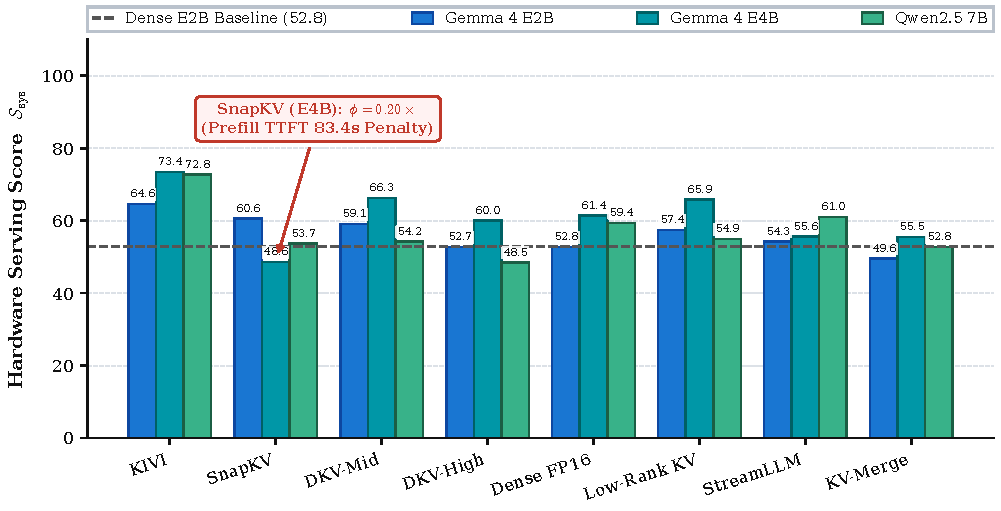
\includegraphics[width=0.92\textwidth]{figures/fig4_ssys_cross.pdf}
\caption{\textbf{Cross-Model Part 2 Hardware System Serving Utility Distribution.} Breakdown of $\mathcal{S}_{\text{sys}}$ across Gemma~4 E2B, Gemma~4 E4B, and Qwen2.5~7B.}
\label{fig:ssys_cross}
\end{figure}

\vspace{-4pt}
\begin{figure}[h]
\centering
\begin{minipage}[t]{0.485\textwidth}
\centering
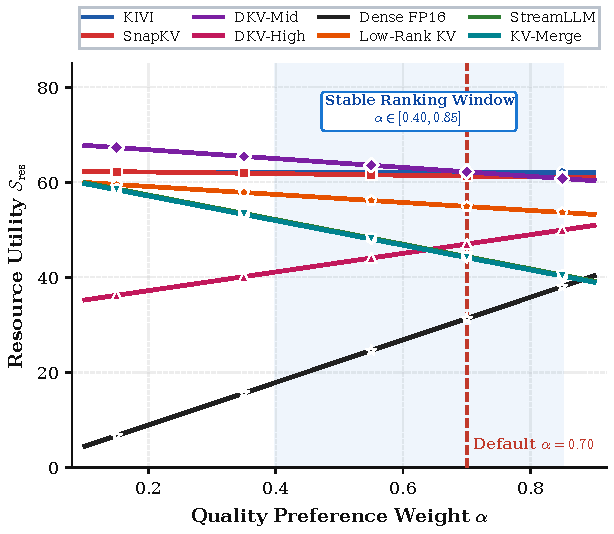
\includegraphics[width=\linewidth]{figures/fig8a_ranking_stability.pdf}
\caption{\textbf{Ranking Stability Across $\alpha$.} Trajectories across $\alpha \in [0.1, 0.9]$.}
\label{fig:alpha_stability}
\end{minipage}\hfill
\begin{minipage}[t]{0.485\textwidth}
\centering
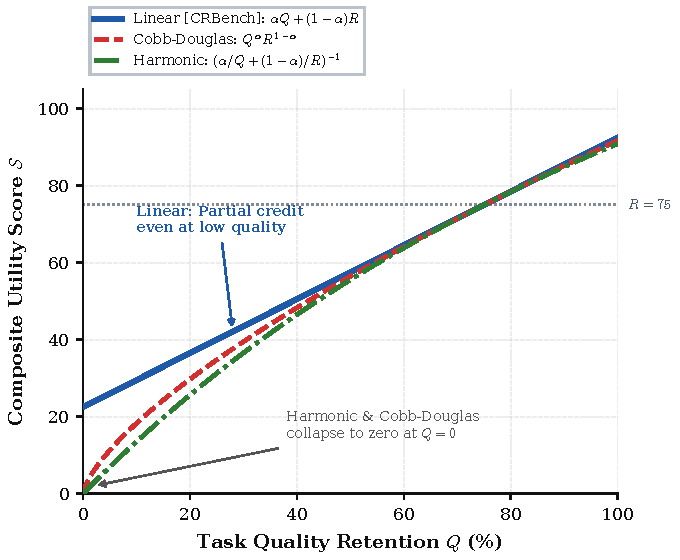
\includegraphics[width=\linewidth]{figures/fig8b_formulation_comparison.pdf}
\caption{\textbf{Utility Formulation Comparison.} Linear vs. Cobb--Douglas vs. Harmonic at $R_{\text{mem}} = 75\%$.}
\label{fig:formulation_comparison}
\end{minipage}
\end{figure}



\end{document}
